%% -*- Lecture -*-

\documentclass[11pt,aspectratio=169]{beamer}

\usepackage{rcstalk}
\usetheme{rcstheme}

\topic{Processes}
%\title{CS350: Processes}

\begin{document}

\maketitle

\tikzstyle{osbox}=[draw, fill=blue!20, text width=20em, text centered, minimum 
height=2em]
\tikzstyle{osbigbox}=[draw, fill=blue!20, text width=25em, text centered, 
minimum height=5em]
\tikzstyle{apibox}=[draw, fill=white, text width=5em, text centered, minimum 
height=2em]
\tikzstyle{hwbox}=[draw, fill=green!20, text width=20em, text centered, minimum 
height=2em]
\tikzstyle{appbox}=[draw, fill=white, text width=5em, text centered, minimum 
height=2em]
\def\blockdist{0.5}

\begin{slide}{Operating System}
\begin{figure}[ht!]
\centering
\begin{tikzpicture}
    \node (os) [osbigbox] {Operating System};
    \path (os.south)+(0,-\blockdist) node (hw) [hwbox] {Hardware: CPU, Memory 
    and Devices};
    \path (os.north)+(0,2*\blockdist) node (emacs) [appbox,fill=yellow!30,text 
    width=20em] {emacs};
\end{tikzpicture}
\end{figure}
\end{slide}

\begin{slide}{Operating System: Basic Abstractions and APIs}
\begin{figure}[ht!]
\centering
\begin{tikzpicture}
    \node (os) [osbigbox] {Operating System};
    \path (os.south)+(0,-\blockdist) node (hw) [hwbox] {Hardware: CPU, Memory 
    and Devices};
    \path (os.north)+(0,2*\blockdist) node (emacs) [appbox,fill=yellow!30,text 
    width=20em] {emacs};
    \path (os.north)+(-9em,0.1) node (procs) [apibox] {Process};
    \path (procs.east)+(1.25,0) node (threads) [apibox] {Threads};
    \path (threads.east)+(1.25,0) node (locks) [apibox] {Locks};
    \path (locks.east)+(1.25,0) node (etc) [apibox] {File I/O};
\end{tikzpicture}
\end{figure}
\end{slide}

\begin{slide}{Today: Introduce the Process Abstraction}
\begin{figure}[ht!]
\centering
\begin{tikzpicture}
    \node (os) [osbigbox] {Operating System};
    \path (os.south)+(0,-\blockdist) node (hw) [hwbox] {Hardware: CPU, Memory 
    and Devices};
    \path (os.north)+(0,2*\blockdist) node (emacs) [appbox,fill=yellow!30,text 
    width=20em] {emacs};
    \path (os.north)+(-9em,0.1) node (procs) [apibox,fill=red!20] {Process};
    \path (procs.east)+(1.25,0) node (threads) [apibox] {Threads};
    \path (threads.east)+(1.25,0) node (locks) [apibox] {Locks};
    \path (locks.east)+(1.25,0) node (etc) [apibox] {File I/O};
\end{tikzpicture}
\end{figure}
\end{slide}

\begin{slide}{Processes}
\itms{
  \item A \emph{process} is an instance of a program running
  \item Examples (can all run simultaneously):
  \ittms{
    \item \texttt{gcc file\_A.c} -- compiler running on file A
    \item \texttt{gcc file\_B.c} -- compiler running on file B
    \item \texttt{emacs} -- text editor
    \item \texttt{firefox} -- web browser
  }
  \item Non-examples (implemented as one process):
  \ittms{
    \item Multiple firefox windows or emacs frames (still one process)
  }
  \item Modern OSes run multiple processes simultaneously
  \item Why processes?
  \ittms{
    \item Simplicity of programming
    \item Higher throughput (better CPU utilization), lower latency
  }
}
\end{slide}

\begin{slide}{Speed}
\vspace{-1em}
\itms{
  \item Multiple processes can increase CPU utilization
  \ittms{
    \item Overlap one process's computation with another's wait
    \item[] 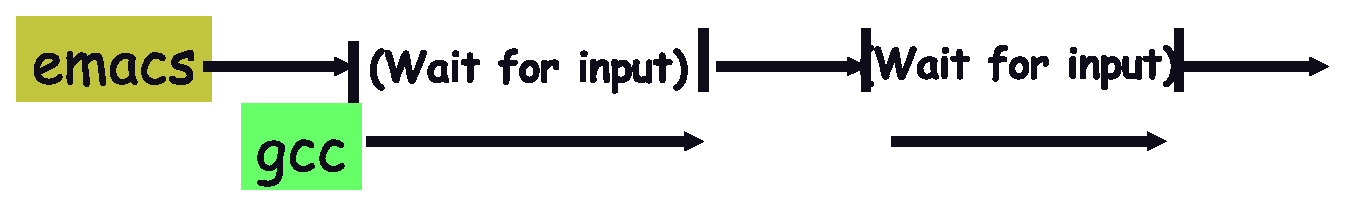
\includegraphics[width=3.5in]{figs/ioparallel}
  }
  \item Multiple processes can reduce latency
  \ittms{
    \item Running $A$ then $B$ requires 100 sec for $B$ to complete \\
     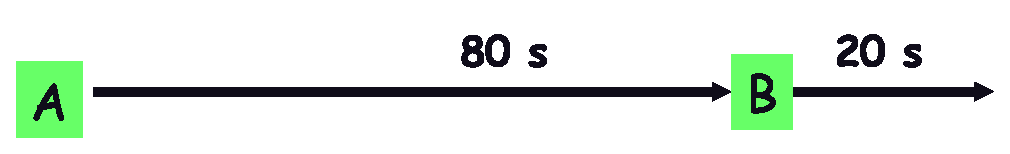
\includegraphics[width=3in]{figs/abseq}
    \item Running $A$ and $B$ concurrently makes $B$ finish faster \\
     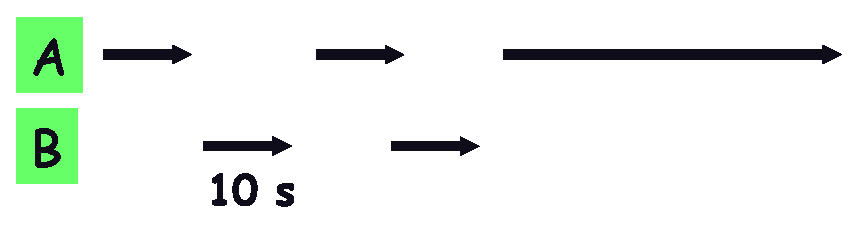
\includegraphics[width=2.5in]{figs/abpar}
   \item $A$ is slower than if it had whole machine to itself,\\
     but still $<100$ sec unless both $A$ and $B$ completely CPU-bound
  }
}
\end{slide}

\begin{slide}{Concurrency and parallelism}
\itms{
  \item Parallelism fact of life much longer than OSes have
	been around
  \ittms{
    \item E.g., say takes 1 worker 10 months to make 1 widget
    \item Company may hire 100 workers to make 100 widgets
    \item Latency for first widget $>\!\!> 1/10$ month
    \item Throughput may be $<10$ widgets per month \\
          (if can't perfectly parallelize task)
    \item And 100 workers making 10,000 widgets may achieve $>10$
      widgets/month
      %\\ (e.g., if workers never idly wait for paint to dry)
  }
  \item Most computers, laptops, and phones are multi-core!
  \item Computer with 4 cores can run 4 processes in parallel
  \item Result: $4\times$ throughput
}
\end{slide}

\begin{slide}{A process's view of the world}
\vspace*{.3in}
\hbox{\begin{minipage}{3.1in}
\itms{
  \item Each process has own view of machine
  \ittms{
    \item Its own address space
    \item Its own open files
    \item Its own virtual CPU (through preemptive multitasking)
  }
  \item \texttt{*(char *)0xc000} different in $P_1$ \& $P_2$
  \item Simplifies programming model
  \ittms{
    \item \texttt{gcc} does not care that \texttt{firefox} is running
    %\item A bug in \texttt{firefox} does not matter to \texttt{gcc}
  }
}
\end{minipage}
\begin{minipage}{1.2in}
\vspace*{-.3in}
\null
\rightline{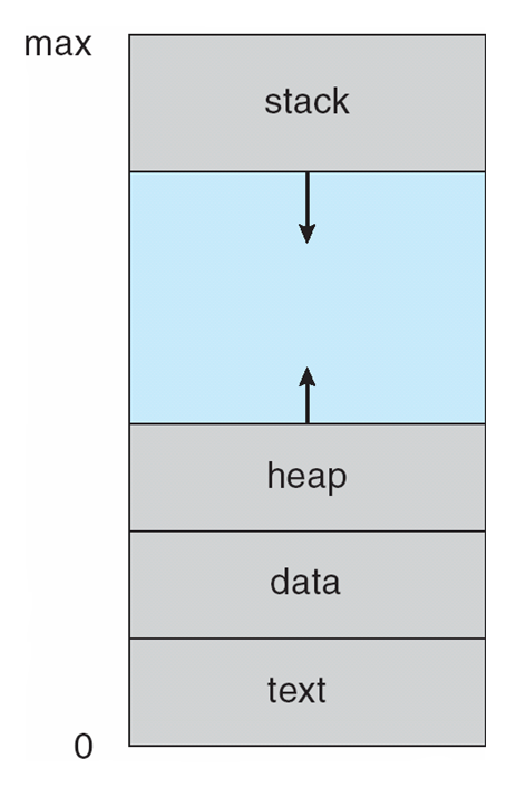
\includegraphics[width=1.3in]{figs/memlayout}}
\end{minipage}}
%\vspace*{-.1in}
\itms{
  \item Sometimes want interaction between processes
  \ittms{
    \item Simplest is through files:  \texttt{emacs} edits file,
  \texttt{gcc} compiles it 
    \item More complicated:  Shell/command, Window manager/app.
  }
}
\end{slide}

\iffalse
\begin{slide}{Inter-Process Communication}
\centerline{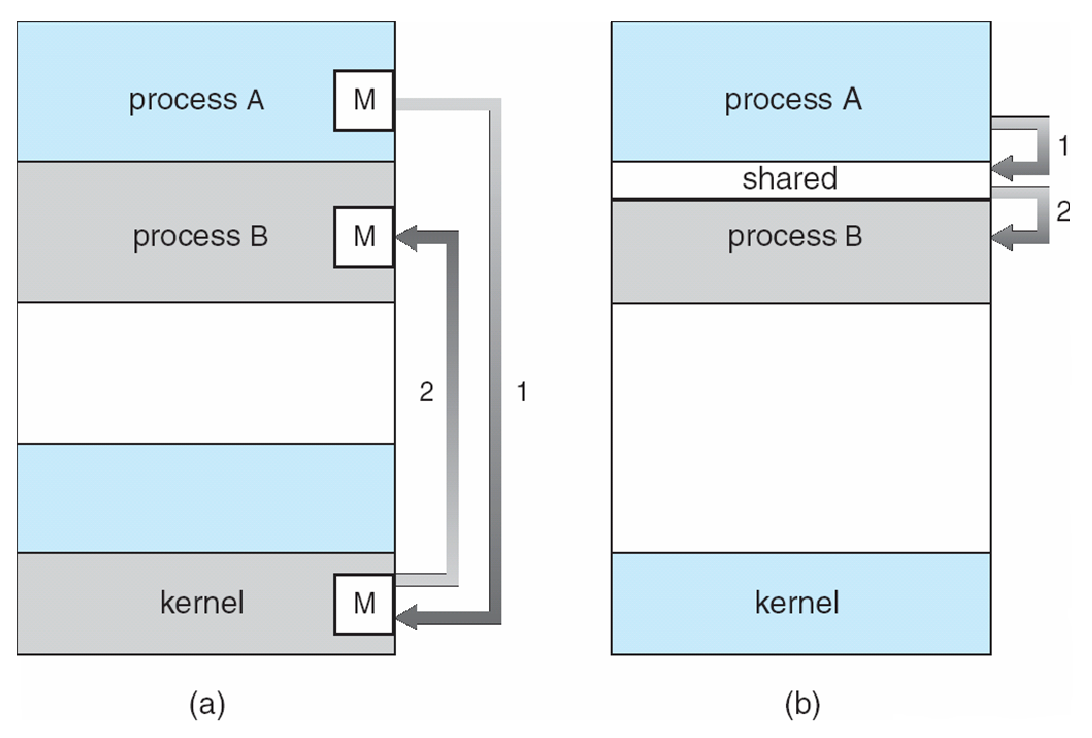
\includegraphics[height=2in]{figs/ipc}}

\small

\itms{
  \item How can processes interact in real time?
  \ittms{
    \item[(a)] By passing messages through the kernel
    \item[(b)] By sharing a region of physical memory
    \item[(c)] Through asynchronous signals or alerts
  }
}
\end{slide}
\fi

\begin{slide}{Rest of lecture}
\itms{
  \item User view of processes
  \ittms{
    \item Crash course in basic Unix/Linux system call interface
    \item How to create, kill, and communicate between processes
    \item Running example: how to implement a shell
  }
  \item Kernel view of processes
  \ittms{
    \item Implementing processes in the kernel
  }
%  \item Threads
%  \item How to implement threads
}
\end{slide}

\section{User view of processes}

%% \begin{slide}{UNIX file I/O}
%% \itms{
%%   \item Applications ``open'' files (or devices) by name
%%   \ittms{
%%     \item I/O happens through open files
%%   }
%%   \item \texttt{int open(char *path, int flags, /*mode*/...);}
%%   \ittms{
%%     \item \texttt{flags}: \texttt{O\_RDONLY}, \texttt{O\_WRONLY},
%% 	\texttt{O\_RDWR}
%%     \item \texttt{O\_CREAT}: create the file if non-existent
%%     \item \texttt{O\_EXCL}: (w.\ \texttt{O\_CREAT}) create if file
%% exists already
%%     \item \texttt{O\_TRUNC}: Truncate the file
%%     \item \texttt{O\_APPEND}: Start writing from end of file
%%     \item \texttt{mode}: final argument with \texttt{O\_CREAT}
%%   }
%%   \item Returns file descriptor---used for all I/O to file
%% }
%% \end{slide}

%% \begin{slide}{Error returns}
%% \itms{
%%   \item What if \texttt{open} fails?  Returns -1 (invalid fd)
%%   \item Most system calls return -1 on failure
%%   \ittms{
%%     \item Specific kind of error in global int \texttt{errno}
%%   }
%%   \item \texttt{\#include <sys/errno.h>} for possible values
%%   \ittms{
%%     \item 2 = \texttt{ENOENT} ``No such file or directory''
%%     \item 13 = \texttt{EACCES} ``Permission Denied''
%%   }
%%   \item \texttt{perror} function prints human-readable message
%%   \ittms{
%%     \item \texttt{perror ("initfile");} \\
%% 	$\to$ ``\texttt{initfile:\ No such file or directory}''
%%   }
%% }
%% \end{slide}

%% \begin{slide}{Operations on file descriptors}
%% \itms{
%%   \item \texttt{int read (int fd, void *buf, int nbytes);}
%%   \ittms{
%%     \item Returns number of bytes read
%%     \item Returns 0 bytes at end of file, or -1 on error
%%   }
%%   \item \texttt{int write (int fd, void *buf, int nbytes);}
%%   \ittms{
%%     \item Returns number of bytes written, -1 on error
%%   }
%%   \item \texttt{off\_t lseek (int fd, off\_t pos, int whence);}
%%   \ittms{
%%     \item \texttt{whence}: 0 -- start, 1 -- current, 2 -- end
%%      \ittms{
%%        \item Returns previous file offset, or -1 on error
%%      }
%%   }
%%   \item \texttt{int close (int fd);}
%% %  \item \texttt{int fsync (int fd);}
%% %  \ittms{
%% %    \item Guarantee that file contents is stably on disk
%% %  }
%% }
%% \end{slide}

%% \begin{slide}{File descriptor numbers}
%% \itms{
%%   \item File descriptors are inherited by processes
%%   \ittms{
%%     \item When one process spawns another, same fds by default
%%   }
%%   \item Descriptors 0, 1, and~2 have special meaning
%%   \ittms{
%%   \item 0 -- ``standard input'' (\texttt{stdin} in ANSI C)
%%   \item 1 -- ``standard output'' (\texttt{stdout, printf} in ANSI C)
%%   \item 2 -- ``standard error'' (\texttt{stderr, perror} in ANSI C)
%%   \item Normally all three attached to terminal
%%   }
%%   \item Example:  \texttt{type.c}
%%   \ittms{
%%     \item Prints the contents of a file to \texttt{stdout}
%%   }
%% }
%% \end{slide}

%% \begin{slide}{\texttt{type.c}}
%% \begin{myverb}
%%          void
%%          typefile (char *filename)
%%          {
%%            int fd, nread;
%%            char buf[1024];

%%            fd = open (filename, O_RDONLY);
%%            if (fd == -1) {
%%              perror (filename);
%%              return;
%%            }

%%            while ((nread = read (fd, buf, sizeof (buf))) > 0)
%%              write (1, buf, nread);

%%            close (fd);
%%          }        
%% \end{myverb}
%% \end{slide}


%% \begin{slide}{The rename system call}
%% \itms{
%%   \item \texttt{int rename (const char *p1, const char *p2);}
%%   \ittms{
%%     \item Changes name \texttt{p2} to reference file \texttt{p1}
%%     \item Removes file name \texttt{p1}
%%   }
%%   \item Guarantees that \texttt{p2} will exist despite any crashes
%%   \ittms{
%%     \item \texttt{p2} may still be old file
%%     \item \texttt{p1} and \texttt{p2} may both be new file
%%     \item but \texttt{p2} will always be old or new file
%%   }
%%   \item \texttt{fsync}/\texttt{rename} idiom used extensively
%%   \ittms{
%%     \item E.g., emacs:  Writes file \texttt{.\#file\#}
%%     \item Calls \texttt{fsync} on file descriptor
%%     \item \texttt{rename (".\#file\#", "file");}
%%   }
%% }
%% \end{slide}

\begin{slide}{Creating processes}
\itms{
  \item \texttt{int \man{fork}(void);}
  \ittms{
    \item Create new process that is exact copy of current one
    \item Returns \textit{process ID} of new process\ in ``parent''
    \item Returns 0 in ``child''
  }
  \item \texttt{int \man{waitpid}(int pid, int *stat, int opt);}
  \ittms{
    \item Wait for a child process to terminate
    \item \texttt{pid} -- process to wait for, or -1 for any
    \item \texttt{stat} -- will contain exit value, or signal
    \item \texttt{opt} -- usually 0 or \texttt{WNOHANG}
    \item Returns process ID or -1 on error
  }
}
\end{slide}

\begin{slide}{Deleting processes}
\itms{
  \item \texttt{void \man{exit}(int status);}
  \ittms{
    \item Current process ceases to exist
    \item \texttt{status} shows up in \texttt{waitpid} (shifted)
    \item By convention, \texttt{status} of 0 is success, non-zero error
  }
  \item \texttt{int \man{kill}(int pid, int sig);}
  \ittms{
    \item Sends signal \texttt{sig} to process \texttt{pid}
    \item \texttt{SIGTERM} most common value, kills process by default \\
          (but application can catch it for ``cleanup'')
    \item \texttt{SIGKILL} stronger, kills process always
  }
}
\end{slide}

\begin{slide}{Running programs}
\vspace*{-.1in}
\itms{
  \item \texttt{int \man{execve}(char *prog, char **argv,
	\hbox to0pt{char **envp);\hss}}
  \ittms{
    \item Execute a new program
    \item \texttt{prog} -- full pathname of program to run
    \item \texttt{argv} -- argument vector that gets passed to \texttt{main}
    \item \texttt{envp} -- environment variables, e.g.,
	\texttt{PATH}, \texttt{HOME}
  }
  \item Generally called through a wrapper functions
  \ittms{
  \item \texttt{int execvp (char *prog, char **argv);} \\
    Search \texttt{PATH} for prog, use current environment
    \item \texttt{int execlp (char *prog, char *arg, ...);}  \\
    List arguments one at a time, finish with \texttt{NULL}
  }
  \item Example: \texttt{minish.c}
  \ittms{
    \item Loop that reads a command, then executes it
  }
}
\end{slide}

\begin{slide}{\texttt{minish.c} (simplified)}
\begin{columns}
    \column{0.4\textwidth}
Parent Process (PID 5)
\begin{smallccode}[numbers=left]
pid_t pid; char **av;
void doexec() {
  execvp(av[0], av);
  perror(av[0]);
  exit(1);
}    

    /* ... main loop: */
    for (;;) {
      parse_input(&av, stdin);
      switch (pid = fork()) {
      case -1:
	perror("fork"); break;
      case 0:
	doexec();
      default:
	waitpid(pid, NULL, 0); break;
      }
    }
\end{smallccode}
\pause
    \column{0.4\textwidth}
Child Process (PID 6)
\begin{smallccode}
pid_t pid; char **av;
void doexec() {
  execvp(av[0], av);
  perror(av[0]);
  exit(1);
}    

    /* ... main loop: */
    for (;;) {
      parse_input(&av, stdin);
      switch (pid = fork()) {
      case -1:
	perror("fork"); break;
      case 0:
	doexec();
      default:
	waitpid(pid, NULL, 0); break;
      }
    }
\end{smallccode}
\end{columns}
\end{slide}

\begin{slide}{\texttt{minish.c} (simplified)}
\begin{columns}
    \column{0.4\textwidth}
Parent Process (PID 5)
\begin{smallccode}[mathescape=true,numbers=left]
pid_t pid; char **av;
void doexec() {
  execvp(av[0], av);
  perror(av[0]);
  exit(1);
}    

    /* ... main loop: */
    for (;;) {
      parse_input(&av, stdin);
      switch (pid = fork()) {
      case -1:
	perror("fork"); break;
      case 0:
	doexec();
      default: // $\leftarrow \textbf{After Fork}~({\tt pid = 6})$
	waitpid(pid, NULL, 0); break;
      }
    }
\end{smallccode}
    \column{0.4\textwidth}
Child Process (PID 6)
    \begin{smallccode}[mathescape=true,]
pid_t pid; char **av;
void doexec() {
  execvp(av[0], av);
  perror(av[0]);
  exit(1);
}    

    /* ... main loop: */
    for (;;) {
      parse_input(&av, stdin);
      switch (pid = fork()) {
      case -1:
	perror("fork"); break;
      case 0: // $\leftarrow \textbf{After Fork}$
	doexec();
      default:
	waitpid(pid, NULL, 0); break;
      }
    }
\end{smallccode}
\end{columns}
\end{slide}

\begin{slide}{\texttt{minish.c} (simplified)}
\begin{columns}
    \column{0.4\textwidth}
Parent Process (PID 5)
\begin{smallccode}[mathescape=true,numbers=left]
pid_t pid; char **av;
void doexec() {
  execvp(av[0], av);
  perror(av[0]);
  exit(1);
}    

    /* ... main loop: */
    for (;;) {
      parse_input(&av, stdin);
      switch (pid = fork()) {
      case -1:
	perror("fork"); break;
      case 0:
	doexec();
      default: // $\leftarrow \textbf{After Fork}~({\tt pid = 6})$
	waitpid(pid, NULL, 0); break;
      }
    }
\end{smallccode}
    \column{0.4\textwidth}
Child Process (PID 6)
    \begin{smallccode}[mathescape=true]
pid_t pid; char **av;
void doexec() {
  execvp(av[0], av); // $\leftarrow \textbf{After Fork}$
  perror(av[0]); // Never executes!
  exit(1);
}

    /* ... main loop: */
    for (;;) {
      parse_input(&av, stdin);
      switch (pid = fork()) {
      case -1:
	perror("fork"); break;
      case 0:
	doexec();
      default:
	waitpid(pid, NULL, 0); break;
      }
    }
\end{smallccode}
\end{columns}
\end{slide}

\begin{slide}{\texttt{minish.c} (simplified)}
\begin{columns}
    \column{0.4\textwidth}
Parent Process (PID 5)
\begin{smallccode}[mathescape=true,numbers=left]
pid_t pid; char **av;
void doexec() {
  execvp(av[0], av);
  perror(av[0]);
  exit(1);
}    

    /* ... main loop: */
    for (;;) {
      parse_input(&av, stdin);
      switch (pid = fork()) {
      case -1:
	perror("fork"); break;
      case 0:
	doexec();
      default: // $\leftarrow \textbf{After Fork}~({\tt pid = 6})$
	waitpid(pid, NULL, 0); break;
      }
    }
\end{smallccode}
    \column{0.4\textwidth}
Child Process (PID 6)
\itms{
    \item Replaced by the new program
}
\begin{smallccode}[mathescape=true]

int
main(int argc, const char *argv[])
{
  // $\leftarrow \textbf{Starts here!}$
  ...
  exit(0);
}
\end{smallccode}
\end{columns}
\end{slide}

\begin{slide}{\texttt{minish.c} (simplified)}
\begin{columns}
    \column{0.4\textwidth}
Parent Process (PID 5)
\begin{smallccode}[mathescape=true,numbers=left]
pid_t pid; char **av;
void doexec() {
  execvp(av[0], av);
  perror(av[0]);
  exit(1);
}    

    /* ... main loop: */
    for (;;) {
      parse_input(&av, stdin);
      switch (pid = fork()) {
      case -1:
	perror("fork"); break;
      case 0:
	doexec();
      default:
	waitpid(pid, NULL, 0); break;
	// $\leftarrow {\tt waitpid}~{\bf returns}$
      }
    }
\end{smallccode}
    \column{0.4\textwidth}
Child Process (PID 6)
\itms{
    \item Replaced by the new program
}
\begin{smallccode}[mathescape=true]

int
main(int argc, const char *argv[])
{

  ...
  exit(0); // $\leftarrow \textbf{Wake up}~{\tt waitpid}$
}
\end{smallccode}
\end{columns}
\end{slide}

\begin{slide}{Manipulating file descriptors}
\itms{
  \item \texttt{int \man{dup2}(int oldfd, int newfd);}
  \ittms{
    \item Closes \texttt{newfd}, if it was a valid descriptor
    \item Makes \texttt{newfd} an exact copy of \texttt{oldfd}
    \item Two file descriptors will share same offset \\
		(\texttt{lseek} on one will affect both)
  }
  \item Example:  \texttt{redirsh.c}
  \ittms{
    \item Loop that reads a command and executes it
    \item Recognizes \texttt{command < input > output 2> errlog}
  }
}
%\rightline{\hyperlink{wfork}{skip 3 slides$\to$}}
\end{slide}

\begin{slide}{\texttt{redirsh.c}}
\vspace{-1em}
\begin{columns}
\column{0.9\textwidth}
\begin{ccode}[numbers=left]
void doexec (void) {
  int fd;
  if (infile) {       /* non-NULL for "command < infile" */
    if ((fd = open(infile, O_RDONLY)) < 0) {
      perror(infile);
      exit(1);
    }
    if (fd != 0) {
      dup2(fd, 0);
      close(fd);
    }
  }

  /* ... do same for outfile`\color{comment}$\to$'fd 1, errfile`\color{comment}$\to$'fd 2 ... */
  execvp (av[0], av);
  perror (av[0]);
  exit (1);
}    
\end{ccode}
\end{columns}
\end{slide}

\begin{slide}{Pipes}
\vspace*{-.1in}
\itms{
  \item \texttt{int \man{pipe}(int fds[2]);}
  \ittms{
    \item Returns two file descriptors in \texttt{fds[0]}
	and \texttt{fds[1]}
    \item Writes to \texttt{fds[1]} will be read on \texttt{fds[0]}
    \item When last copy of \texttt{fds[1]} closed, \texttt{fds[0]}
		will return EOF
    \item Returns 0 on success, -1 on error
  }
  \item Operations on pipes
  \ittms{
    \item \texttt{read}/\texttt{write}/\texttt{close} -- as with files
    \item When \texttt{fds[1]} closed, \texttt{read(fds[0])} returns 0 bytes
    \item When \texttt{fds[0]} closed, \texttt{write(fds[1])}:
    \ittms{
      \item Kills process with \texttt{SIGPIPE}
      \item Or if signal ignored, fails with EPIPE
    }
  }
  \item Example: \texttt{pipesh.c}
  \ittms{
    \item Sets up pipeline \texttt{command1 | command2 | command3 ...}
  }
}
\end{slide}

\begin{slide}{\texttt{pipesh.c} (simplified)}
\vspace{-1em}
\begin{columns}
\column{0.9\textwidth}
\begin{ccode}[numbers=left,basicstyle=\ttfamily\openup-.6\jot]
void doexec (void) {
  while (outcmd) {
    int pipefds[2]; pipe(pipefds);
    switch (fork()) {
    case -1:
      perror("fork"); exit(1);
    case 0:
      dup2(pipefds[1], 1);
      close(pipefds[0]); close(pipefds[1]);
      outcmd = NULL;
      break;
    default:
      dup2(pipefds[0], 0);
      close(pipefds[0]); close(pipefds[1]);
      parse_input(&av, &outcmd, outcmd);
      break;
    }
  }
\end{ccode}
\end{columns}
\end{slide}

\begin{slide}{\hypertarget{wfork}{Why fork?}}
\itms{
  \item Most calls to \texttt{fork} followed by \texttt{execve}
  \item Could also combine into one \emph{spawn} system call
  \item Occasionally useful to fork one process
  \ittms{
    \item Pre-forked Webservers for parallelism
    \item Creates one process per core to serve clients
    \item Lots of uses: Nginx, PostgreSQL, etc.
    %\item Unix \emph{dump} utility backs up file system to tape
    %\item If tape fills up, must restart at some logical point
    %\item Implemented by forking to revert to old state if tape ends
  }
  \item Real win is simplicity of interface
  \ittms{
    \item Tons of things you might want to do to child: \\
          Manipulate file descriptors, environment, resource limits, etc.
    \item Yet \texttt{fork} requires \emph{no} arguments at all
  }
}
\end{slide}

\begin{slide}{Spawning process w/o fork}
\itms{
  \item Without fork, require tons of different options
  \item Example:  Windows
    \href{http://msdn.microsoft.com/en-us/library/ms682425(v=VS.85).aspx}{\texttt{CreateProcess}}
        system call
  \ittms{
    \item Also
      \href{http://msdn.microsoft.com/en-us/library/ms682429(v=VS.85).aspx}%
           {\texttt{CreateProcessAsUser}},
      \href{http://msdn.microsoft.com/en-us/library/ms682431(v=VS.85).aspx}%
           {\texttt{CreateProcessWithLogonW}},
      \href{http://msdn.microsoft.com/en-us/library/ms682434(v=VS.85).aspx}%
           {\texttt{CreateProcessWithTokenW}},
      \ldots
  }
}

\bigskip

\begin{ccode}
BOOL WINAPI CreateProcess(
  _In_opt_       LPCTSTR lpApplicationName,
  _Inout_opt_    LPTSTR lpCommandLine,
  _In_opt_       LPSECURITY_ATTRIBUTES lpProcessAttributes,
  _In_opt_       LPSECURITY_ATTRIBUTES lpThreadAttributes,
  _In_           BOOL bInheritHandles,
  _In_           DWORD dwCreationFlags,
  _In_opt_       LPVOID lpEnvironment,
  _In_opt_       LPCTSTR lpCurrentDirectory,
  _In_           LPSTARTUPINFO lpStartupInfo,
  _Out_          LPPROCESS_INFORMATION lpProcessInformation
);
\end{ccode}
\end{slide}

\section{Kernel view of processes}

\begin{slide}{Implementing processes}
\begin{columns}[c]
    \column{.7\textwidth}
\vspace*{-1mm}
  \itms{
  \item OS keeps data structure for each proc
  \ittms{
    \item Process Control Block (PCB)
    \item Called \texttt{proc} in Unix, \texttt{task\_struct} in
      Linux, and \texttt{struct Process} in COS
  }
  \item Tracks \emph{state} of the process
  \ittms{
    \item Running, ready (runnable), blocked, etc.
  }
  \item Includes information necessary to run
  \ittms{
    \item Registers, virtual memory mappings, etc.
    \item Open files (including memory mapped files)
  }
  \item Various other data about the process
  \ittms{
    \item Credentials (user/group ID), signal mask, controlling
  terminal, priority, accounting statistics, whether being
  debugged, which system call binary emulation in use, \ldots
  }
  }
    \column{.33\textwidth}
    \centerline{\input{pcb}}
    \centerline{PCB}
\end{columns}
\end{slide}

\begin{slide}{Process states}
\centerline{\includegraphics[width=3.0in]{procstate}}

\itms{
  \item Process can be in one of several states
  \ittms{
    \item \emph{new} \& \emph{terminated} at beginning \& end of life
    \item \emph{running} -- currently executing (or will execute on
  kernel return)
    \item \emph{ready} -- can run, but kernel has chosen different
	  process to run
    \item \emph{waiting} -- needs async event (e.g., disk operation) to
  proceed
  }
  \item Which process should kernel run?
  \ittms{
    \item if 0 runnable, run idle loop (or halt CPU), if 1 runnable, run it
    \item if $>$1 runnable, must make scheduling decision
  }
}
\end{slide}

\begin{slide}{Scheduling}
\itms{
\item How to pick which process to run
\item Scan process table for first runnable?
\ittms{
  \item Expensive.  Weird priorities (small pids do better)
  \item Divide into runnable and blocked processes
}
\item FIFO/Round-Robin?
\ittms{
  \item Put threads on back of list, pull them from front \\
  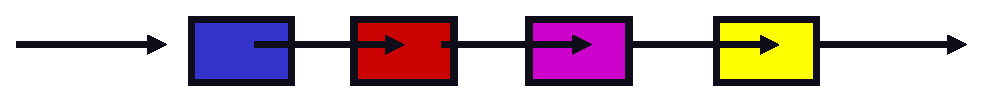
\includegraphics[width=2.5in]{figs/proclist} \\
  (COS \texttt{sys/kern/sched.c})
}
\item Priority?
\ittms{
  \item Give some threads a better shot at the CPU
}
}
\end{slide}

\iffalse
\begin{slide}{Scheduling policy}
\itms{
  \item Want to balance multiple goals
  \ittms{
    \item \emph{Fairness} -- don't starve processes
    \item \emph{Priority} -- reflect relative importance of procs
    \item \emph{Deadlines} -- must do $x$ (play audio) by certain time
    \item \emph{Throughput} -- want good overall performance
    \item \emph{Efficiency} -- minimize overhead of scheduler itself
  }
  \item No universal policy
  \ittms{
    \item Many variables, can't optimize for all
    \item Conflicting goals (e.g., throughput or priority vs.\ fairness)
  }
  %\item We will spend a whole week on this topic
  \item We will spend a whole lecture on this topic
}
\end{slide}
\fi

\begin{slide}{Preemption}
\itms{
  \item Can preempt a process when kernel gets control
  \item Running process can vector control to kernel
  \ittms{
    \item System call, page fault, illegal instruction, etc.
    \item May put current process to sleep---e.g., read from disk
    \item May make other process runnable---e.g., fork, write to pipe
  }
  \item Periodic timer interrupt
  \ittms{
    \item If running process used up quantum, schedule another
  }
  \item Device interrupt
  \ittms{
    \item Disk request completed, or packet arrived on network
    \item Previously waiting process becomes runnable
    \item Schedule if higher priority than current running proc.
  }
  \item Changing running process is called a \emph{context switch}
}
\end{slide}

\begin{slide}{Context switch}
\centerline{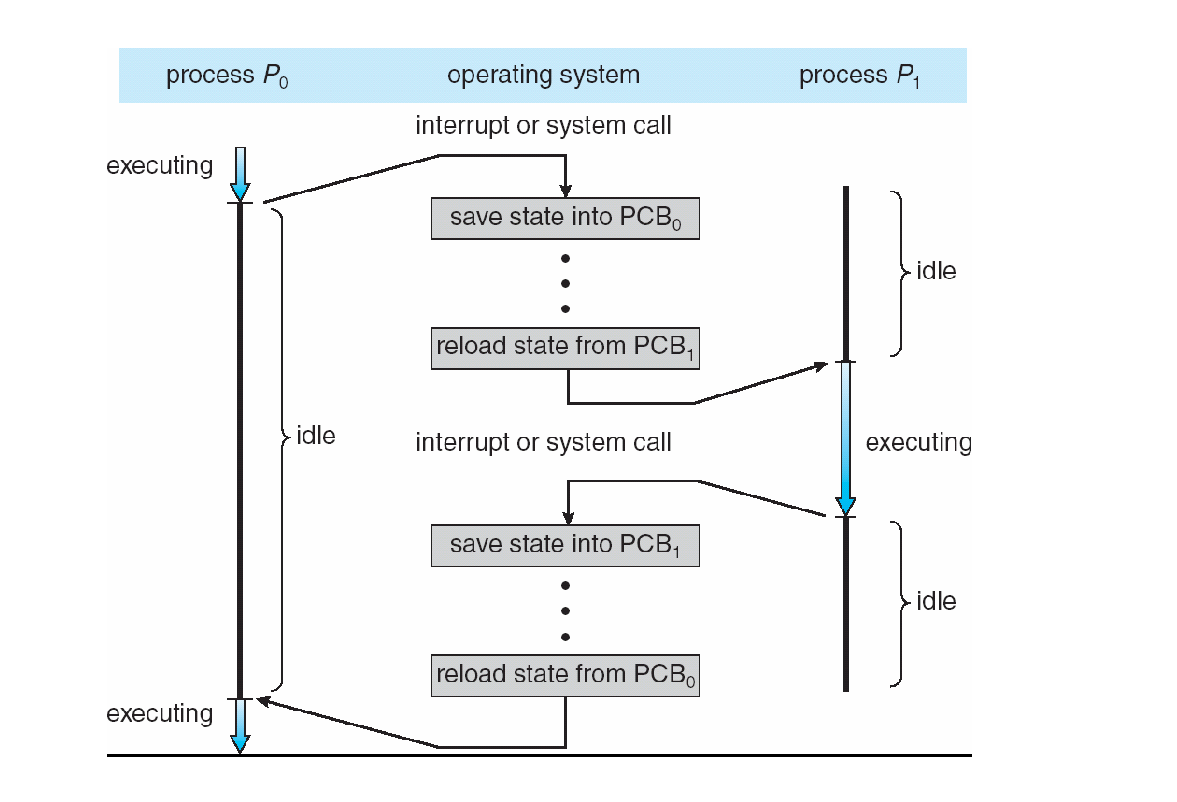
\includegraphics[height=70mm]{figs/switch}}
\end{slide}

\begin{slide}{Context switch details}
\itms{
  \item Very machine dependent.  Typical things include:
  \ittms{
    \item Save program counter and integer registers (always)
    \item Save floating point or other special registers
    \item Save condition codes
    \item Change virtual address translations
  }
  \item Non-negligible cost
  \ittms{
    \item Save/restore floating point registers expensive \\
    \itttms{
      \item Optimization: only save if process used floating point
    }
    \item May require flushing TLB (memory translation hardware) \\
    \itttms{
      \item HW Optimization~1: don't flush kernel's own data from TLB
      \item HW Optimization~2: use tag to avoid flushing any data
    }
    \item Usually causes more cache misses (switch working sets)
  }
}
\end{slide}

\iffalse
\section{Threads}

\begin{slide}{Threads}
\centerline{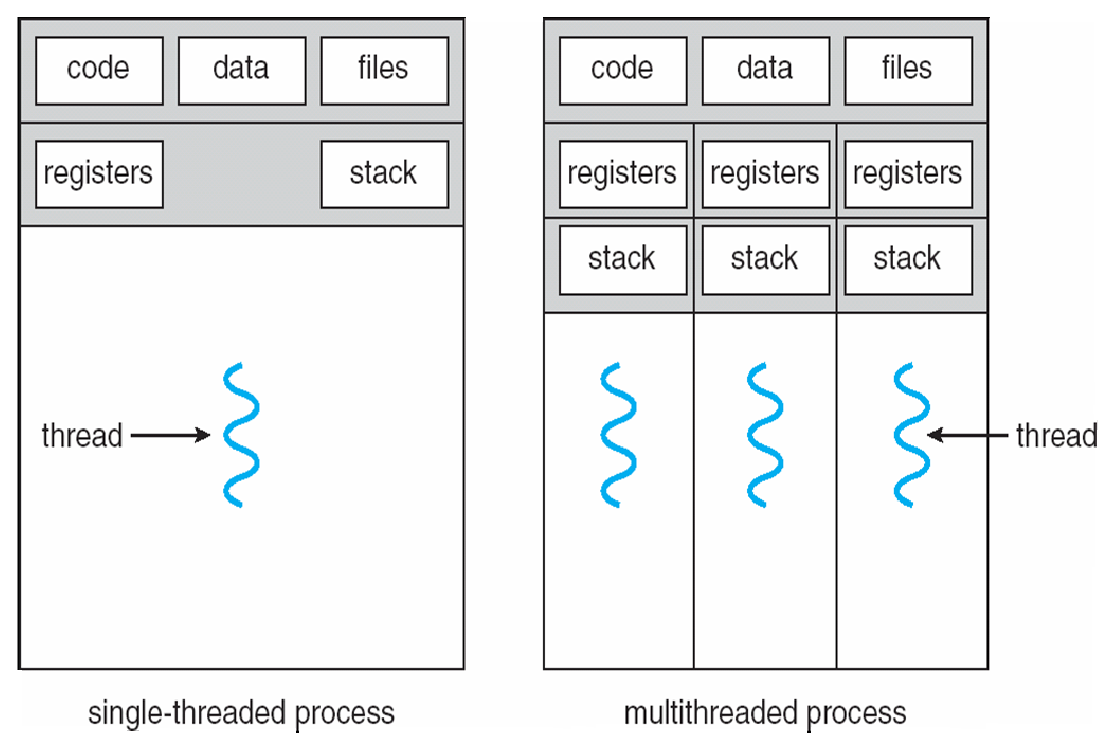
\includegraphics[height=53mm]{figs/thread}}
\itms{
  \item A thread is a schedulable execution context
  \ittms{
    \item Program counter, stack, registers, \ldots
  }
  \item Simple programs use one thread per process
  \item But can also have multi-threaded programs
  \ittms{
    \item Multiple threads running in same process's address space
  }
}
\end{slide}

\begin{slide}{Why threads?}
\itms{
  \item Most popular abstraction for concurrency
  \ittms{
    \item Lighter-weight abstraction than processes
    \item All threads in one process share memory, file descriptors, etc.
  }
  \item Allows one process to use multiple CPUs or cores
  \item Allows program to overlap I/O and computation
  \ittms{
    \item Same benefit as OS running \texttt{emacs} \& \texttt{gcc}
	    simultaneously
    \item E.g., threaded web server services clients simultaneously:
  }
}
\vspace*{-1ex}
\begin{ccode}
        for (;;) {
          fd = accept_client ();
          thread_create (service_client, &fd);
        }
\end{ccode}
\itms{
  \item Most kernels have threads, too
  \ittms{
    \item Typically at least one kernel thread for every process
  }
}
\end{slide}


\begin{slide}{Thread package API}
\itms{
  \item \texttt{tid thread\_create (void (*fn) (void *), void *);}
  \ittms{
    \item Create a new thread, run \texttt{fn} with \texttt{arg}
  }
  \item \texttt{void thread\_exit ();}
  \ittms{
    \item Destroy current thread
  }
  \item \texttt{void thread\_join (tid thread);}
  \ittms{
    \item Wait for thread \texttt{thread} to exit
  }
  \item Plus lots of support for synchronization [in 3 weeks]
  \item See \cref{sched/readings/birrell.pdf}{[Birell]} for good
    introduction
  \item Can have preemptive or non-preemptive threads
  \ittms{
    \item Preemptive causes more race conditions
    \item Non-preemptive can't take advantage of multiple CPUs
    \item Before prevalent SMPs, most kernels non-preemptive
  }
}
\end{slide}


\begin{slide}{Kernel threads}

\centerline{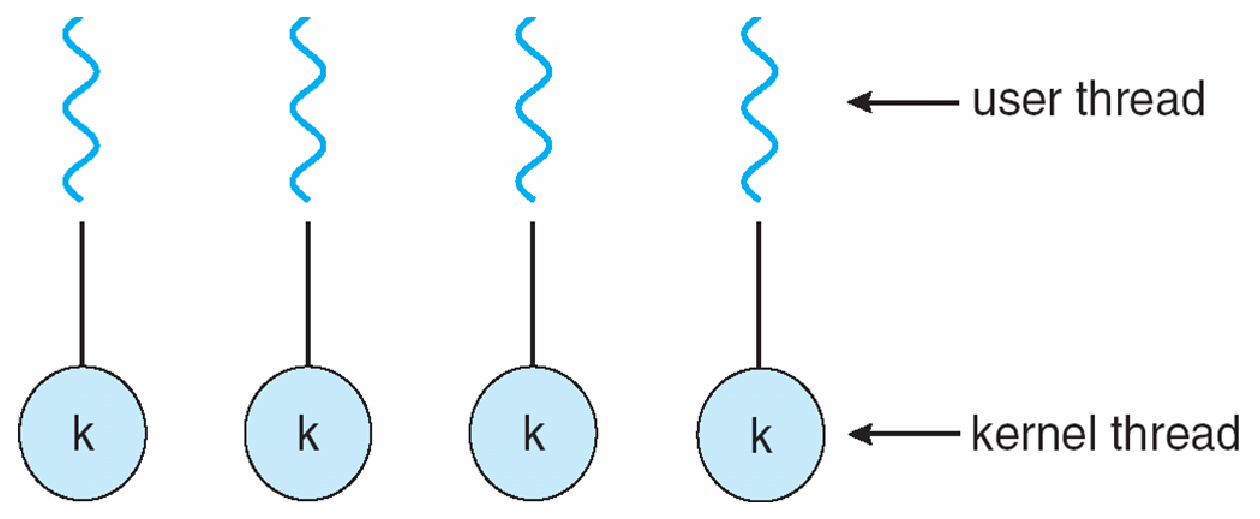
\includegraphics[height=32mm]{figs/kthread}}

\itms{
  \item Can implement \texttt{thread\_create} as a system call
  \item To add \texttt{thread\_create} to an OS that doesn't have it:
  \ittms{
    \item Start with process abstraction in kernel
    \item \texttt{thread\_create} like process creation with features
      stripped out
    \itttms{
      \item Keep same address space, file table, etc., in new process
      \item \texttt{rfork}/\texttt{clone} syscalls actually allow individual control
    }
  }
  \item Faster than a process, but still very heavy weight
}
\end{slide}

\begin{slide}{Limitations of kernel-level threads}
\itms{
  \item Every thread operation must go through kernel
  \ittms{
    \item create, exit, join, synchronize, or switch for any reason
    \item On my laptop: syscall takes 100 cycles, fn call 5 cycles
    \item Result: threads 10x-30x slower when implemented in kernel
  }
  \item One-size fits all thread implementation
  \ittms{
    \item Kernel threads must please all people
    \item Maybe pay for fancy features (priority, etc.) you don't need
  }
  \item General heavy-weight memory requirements
  \ittms{
    \item E.g., requires a fixed-size stack within kernel
    \item Other data structures designed for heavier-weight processes
  }
}
\end{slide}

\begin{slide}{User threads}
\centerline{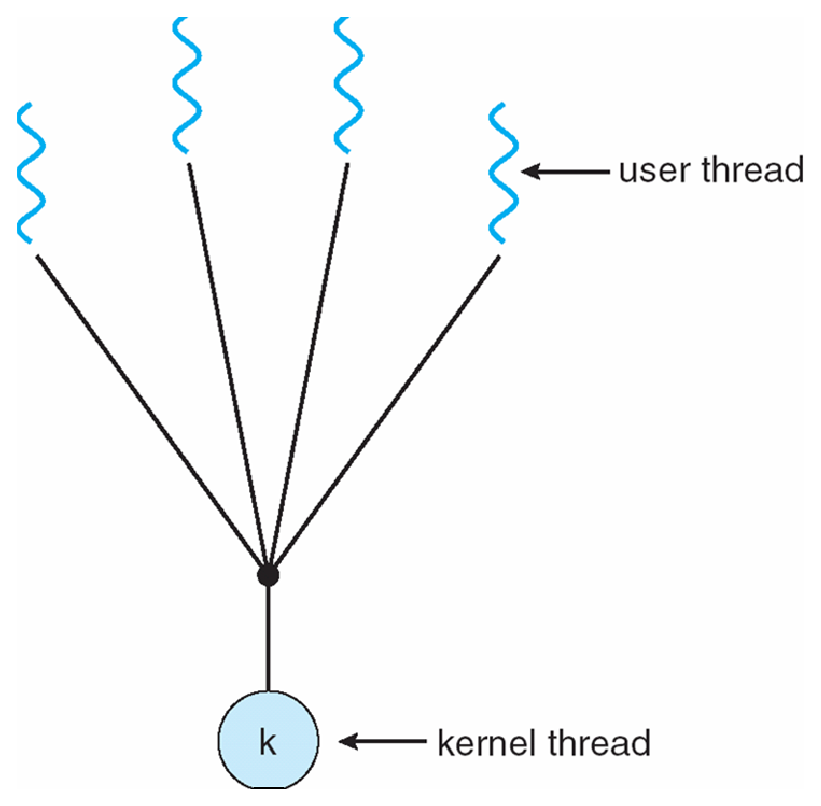
\includegraphics[height=64mm]{figs/uthread}}
\itms{
  \item An alternative: implement in user-level library
  \ittms{
    \item One kernel thread per process
    \item \texttt{thread\_create}, \texttt{thread\_exit}, etc., just library functions
  }
}
\end{slide}

\begin{slide}{Implementing user-level threads}
\itms{
  \item Allocate a new stack for each \texttt{thread\_create}
  \item Keep a queue of runnable threads
  \item Replace networking system calls (\texttt{read}/\texttt{write}/etc.)
  \ittms{
    \item If operation would block, switch and run different thread
  }
  \item Schedule periodic timer signal (\texttt{setitimer})
  \ittms{
    \item Switch to another thread on timer signals (preemption)
  }
  \item Multi-threaded web server example
  \ittms{
    \item Thread calls \texttt{read} to get data from remote web browser
    \item ``Fake'' \texttt{read} \emph{function} makes \texttt{read}
      \emph{syscall} in non-blocking mode
    \item No data?  schedule another thread
    \item On timer or when idle check which connections have new data
  }
  %\item How to switch threads?
}
\end{slide}

\section{How to implement threads}

\begin{slide}{Background: calling conventions}
\begin{columns}
\column{.67\textwidth}   
\itms{
  \item Registers divided into 2 groups
  \ittms{
    \item Functions free to clobber \Red{\emph{caller-saved}}
      \rlap{regs} \\
      (\texttt{\%eax} [return val], \texttt{\%edx}, \& \texttt{\%ecx}
      on \rlap{x86)}
    \item But must restore \Red{\emph{callee-saved}} ones to
      original value upon return (on x86, \texttt{\%ebx},
      \texttt{\%esi}, \texttt{\%edi}, plus \texttt{\%ebp} and
      \texttt{\%esp})
  }
  \item \emph{sp} register always base of stack
  \ittms{
    \item Frame pointer (\emph{fp}) is old \emph{sp}
  }
  \item Local variables stored in registers and on stack
  \item Function arguments go in caller-saved regs and on stack
  \ittms{
    \item With x86, all arguments on stack
  }
}
\column{.4\textwidth}
\input{stkframe.tex}
\end{columns}
\end{slide}

\begin{slide}{Background: procedure calls}
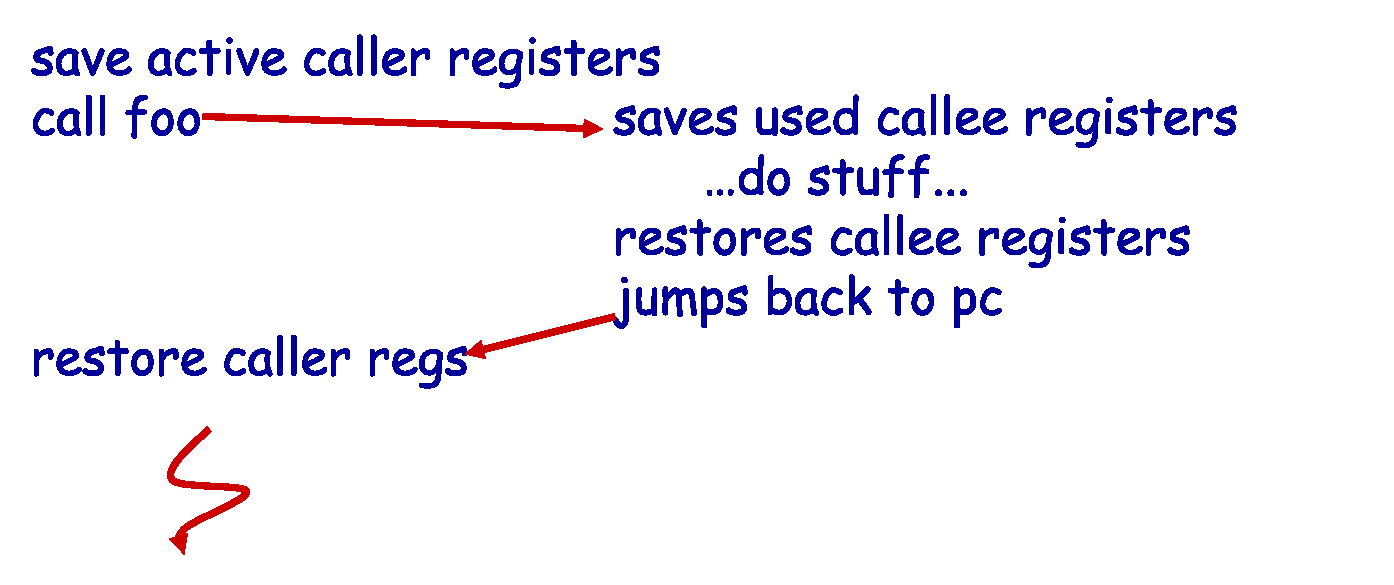
\includegraphics[height=48mm]{figs/proc}
\itms{
  \item Some state saved on stack
  \ittms{
    \item Return address, caller-saved registers
  }
  \item Some state not saved
  \ittms{
    \item Callee-saved regs, global variables, stack pointer
  }
}
\end{slide}

\begin{slide}{Threads vs.\ procedures}
\itms{
\item Threads may resume out of order: 
\ittms{
  \item Cannot use LIFO stack to save state
  \item General solution: one stack per thread
}
\item Threads switch less often:
\ittms{
  \item Don't partition registers (why?)
}
\item Threads can be involuntarily interrupted:
\ittms{
  \item Synchronous: procedure call can use compiler to save state
  \item Asynchronous: thread switch code saves all registers
}
\item More than one than one thread can run at a time:
\ittms{
  \item Procedure call scheduling obvious: Run called procedure
  \item Thread scheduling: What to run next and on which CPU?  
}
}
\end{slide}

\begin{slide}{Example user threads implementation}
\itms{
  \item Per-thread state in thread control block structure
}
{%
\begin{ccode}
    typedef struct tcb {
      uintptr_t long md_esp;    /* Stack pointer of thread */
      char *t_stack;            /* Bottom of thread's stack */
      /* ... */
    };  
\end{ccode}}
\itms{
  \item Machine-dependent thread-switch function:
  \ittms{
    \item \normalsize\texttt{void thread\_md\_switch (tcb *\Green{current}, tcb
*\Magenta{next});}
  }
  \item Machine-dependent thread initialization function:
  \ittms{
    \item \normalsize\texttt{void thread\_md\_init (tcb *t,
	void (*fn) (void *),\break\null\qquad void *arg);}
  }
}
\end{slide}

\defverbatim[colored]\threadswitch{\small%
\begin{asm}
pushl %ebp; movl %esp,%ebp             # Save frame pointer
pushl %ebx; pushl %esi; pushl %edi     # Save callee-saved regs

movl 8(%ebp),%edx                      # %edx = thread_current
movl 12(%ebp),%eax                     # %eax = thread_next
movl %esp,(%edx)                       # %edx->md_esp = %esp
movl (%eax),%esp                       # %esp = %eax->md_esp

popl %edi; popl %esi; popl %ebx        # Restore callee saved regs
popl %ebp                              # Restore frame pointer
ret                                    # Resume execution
\end{asm}
}

\begin{frame}[fragile]
\frametitle{i386 thread\_md\_switch}
\medskip
\begin{overlayarea}{\textwidth}{56mm}%
\only<1>{\threadswitch}%
\only<2>{\centerline{\input{switch1}}}%
\only<3>{\centerline{\input{switch2}}}%
\only<4>{\centerline{\input{switch3}}}%
\only<5>{\centerline{\input{switch4}}}%
\only<6>{\centerline{\input{switch5}}}%
\end{overlayarea}
\smallskip
\itms{
  \item This is literally switch code from simple thread library
  \ittms{
    \item Nothing magic happens here
  \item You will see very similar code in COS \texttt{kern/amd64/switch.S}
  }
}
\end{frame}

\begin{slide}{Limitations of user-level threads}
\itms{
  \item Can't take advantage of multiple CPUs or cores
  \item A blocking system call blocks all threads
  \ittms{
    \item Can replace \texttt{read} to handle network connections
    \item But usually OSes don't let you do this for disk
    \item So one uncached disk read blocks all threads
  }
  \item A page fault blocks all threads
  \item Possible deadlock if one thread blocks on another
  \ittms{
    \item May block entire process and make no progress
    \item {}[More on deadlock in future lectures.]
  }
}
\end{slide}

\begin{slide}{User threads on kernel threads}
\centerline{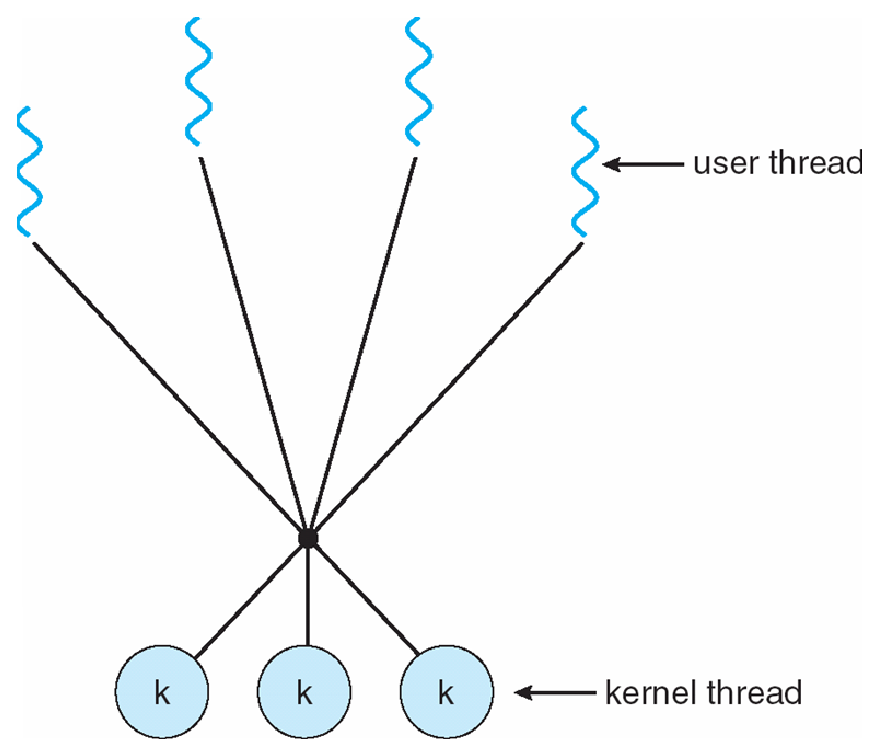
\includegraphics[height=1.9in]{figs/ukthread}}
\itms{
  \item User threads implemented on kernel threads
  \ittms{
    \item Multiple kernel-level threads per process
    \item \texttt{thread\_create}, \texttt{thread\_exit}
      still library functions as before
  }
  \item Sometimes called $n:m$ threading
  \ittms{
    \item Have $n$ user threads per $m$ kernel threads \\
      (Simple user-level threads are $n:1$, kernel threads $1:1$)
  }
}
\end{slide}

\begin{slide}{Limitations of $n:m$ threading}
\itms{
  \item Many of same problems as $n:1$ threads
  \ittms{
    \item Blocked threads, deadlock, \ldots
  }
  \item Hard to keep same \# kthreads as available CPUs
  \ittms{
    \item Kernel knows how many CPUs available
    \item Kernel knows which kernel-level threads are blocked
    \item But tries to hide these things from applications for
      transparency
    \item So user-level thread scheduler might think a thread is
      running while underlying kernel thread is blocked
  } 
  \item Kernel doesn't know relative importance of threads
  \ittms{
    \item Might preempt kthread in which library holds important lock
  }
}
\end{slide}

\begin{slide}{Lessons}
\itms{
  \item Threads best implemented as a library
  \ittms{
    \item But kernel threads not best interface on which to do this
  }
  \item Better kernel interfaces have been suggested
  \ittms{
    \item See Scheduler Activations
\href{http://www.cs.washington.edu/homes/tom/pubs/sched_act.pdf}{[Anderson et al.]}
    \item Maybe too complex to implement on
      existing OSes (some have added then removed such features, now
      Windows is trying it)
  }
  \item Today shouldn't dissuade you from using threads
  \ittms{
    \item Standard user or kernel threads are fine for most purposes
    \item Use kernel threads if I/O concurrency main goal
    \item Use $n:m$ threads for highly concurrent (e.g,. scientific
 applications) with many thread switches
  }
  \item \ldots though concurrency/synchronization lectures may
  \ittms{
    \item Concurrency greatly increases the complexity of a program!
    \item Leads to all kinds of nasty race conditions
  }
}
\end{slide}

\section{OS/161}
\begin{slide}{OS/161 Differences}
\begin{ccode}
int thread_fork(const char *name,
  struct proc *proc,
  void (*entrypoint)(void *data1, unsigned long data2),
  void *data1, unsigned long data2);
\end{ccode}
\itms{
  \item OS/161 supports fork, exec, exit, and wait
  \ittms{
    \item You will implement these functions in Assignments 2a/2b
  }
  \item OS/161 only contains thread in the kernel
  \item One thread per process
  \item To create a thread call: \texttt{thread\_fork()}
  \item Don't be confused it is just another variant of thread\_create!
}
\end{slide}

\fi

\end{document}
